% \documentclass[UTF8,oneside]{ctexbook}
% \usepackage{pgfplots}
% \usepackage{caption}
% \begin{document}

\begin{figure}[!h]
\centering
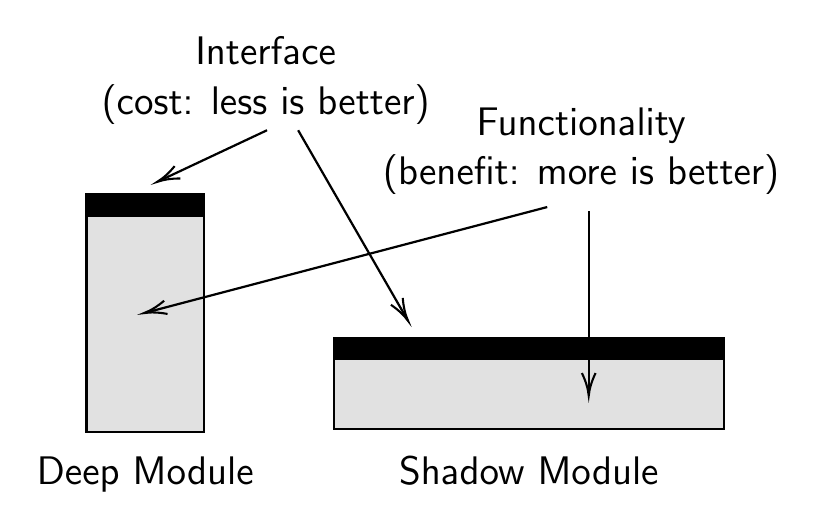
\begin{tikzpicture}[
    x=0.75pt,y=0.75pt,
    yscale=-1,xscale=1,
    font = \sffamily\Large,
    every path/.append style ={line width = 0.8pt,},
]
    
    % 矩形
    \draw [
        fill = {rgb, 255:red, 155; green, 155; blue, 155 },
        fill opacity=0.3 
    ] (42.67,94) -- (99.33,94) -- (99.33,208.68) -- (42.67,208.68) -- cycle ;
    \draw [
        fill = {rgb, 255:red, 0; green, 0; blue, 0 },
        fill opacity=1 
    ] (42.67,94) -- (99.33,94) -- (99.33,104.32) -- (42.67,104.32) -- cycle ;
    
    \draw [
        fill={rgb, 255:red, 155; green, 155; blue, 155 },
        fill opacity=0.3 
    ] (162,163.32) -- (349.65,163.32) -- (349.65,207.32) -- (162,207.32) -- cycle ;
    \draw [
        fill={rgb, 255:red, 0; green, 0; blue, 0 },
        fill opacity=1 
    ] (162,173.32) -- (349.65,173.32) -- (349.65,163.32) -- (162,163.32) -- cycle ;
    
    % 箭头
    \draw (129.65,63.23) -- (78.46,87.29) ;
    \draw [shift={(76.65,88.14)}, rotate = 334.83] [color={rgb, 255:red, 0; green, 0; blue, 0 }  ][line width=0.75]    (10.93,-3.29) .. controls (6.95,-1.4) and (3.31,-0.3) .. (0,0) .. controls (3.31,0.3) and (6.95,1.4) .. (10.93,3.29)   ;
    \draw (144.65,63.23) -- (196.65,153.4) ;
    \draw [shift={(197.65,155.14)}, rotate = 240.03] [color={rgb, 255:red, 0; green, 0; blue, 0 }  ][line width=0.75]    (10.93,-3.29) .. controls (6.95,-1.4) and (3.31,-0.3) .. (0,0) .. controls (3.31,0.3) and (6.95,1.4) .. (10.93,3.29)   ;
    \draw (264.65,100.23) -- (72.26,150.83) ;
    \draw [shift={(70.33,151.34)}, rotate = 345.26] [color={rgb, 255:red, 0; green, 0; blue, 0 }  ][line width=0.75]    (10.93,-3.29) .. controls (6.95,-1.4) and (3.31,-0.3) .. (0,0) .. controls (3.31,0.3) and (6.95,1.4) .. (10.93,3.29)   ;
    \draw (284.65,102.23) -- (284.65,189.14) ;
    \draw [shift={(284.65,191.14)}, rotate = 270] [color={rgb, 255:red, 0; green, 0; blue, 0 }  ][line width=0.75]    (10.93,-3.29) .. controls (6.95,-1.4) and (3.31,-0.3) .. (0,0) .. controls (3.31,0.3) and (6.95,1.4) .. (10.93,3.29)   ;
    
    % 文本
    \draw (129,39.32)       node [align=center] { 
        Interface\\(cost: less is better)
    };
    \draw (281,73.32)       node [align=center] {
        Functionality\\(benefit: more is better)
    };
    \draw (71,229.32)       node [align=left] {Deep Module};
    \draw (255.83,227.32)   node [align=left] {Shadow Module};
\end{tikzpicture}
\caption*{图 4.1}
\label{fig:4-1}
\end{figure}

% \end{document}